\UseRawInputEncoding
\documentclass[pdflatex,sn-mathphys]{sn-jnl}
\usepackage{graphicx}
\usepackage{amsmath}
\usepackage{amsfonts}
\usepackage{array}
\usepackage{siunitx}
\usepackage{bookmark}
\usepackage{natbib,hyperref}
\setcitestyle{round}
\usepackage{gensymb}
%\usepackage{authblk}
\usepackage{textgreek}
\usepackage{caption}
% Deze hieronder zorgt dat plaatjes binnen section blijven
%\usepackage[section]{placeins}
%\usepackage{fancyref}
%\usepackage{ccaption}
%\captionsetup[table]{position=below}
\sisetup{
    exponent-product = \cdot,
    range-phrase = -,
    range-units = single,
    detect-weight = true,
    detect-family = true,
    detect-all = true}

\jyear{2022}
\raggedbottom
%\newcommand{\makeAlph}[1]{\@alph{#1}}

\begin{document}

\newcommand{\red}{\textcolor{red}}


\title{\centering Measuring gravity with milligram levitated masses}

\author[1]{\fnm{Tim M.} \sur{Fuchs}}
\author[1]{\fnm{Dennis G.} \sur{Uitenbroek}}
\author[1]{\fnm{Jaimy} \sur{Plugge}}
\author[1]{\fnm{Noud} \sur{van Halteren}}
\author[1]{\fnm{Jean-Paul} \sur{van Soest}}
\author[3]{\fnm{Andrea} \sur{Vinante}} %er mag hier geen spatie bij de "2,3" want dan krijgt hij superscript 2,1 ipv 2,3 Thanks!
\author[2]{\fnm{Hendrik} \sur{Ulbricht}}
\author*[1]{\fnm{Tjerk H.} \sur{Oosterkamp}}\email{oosterkamp@physics.leidenuniv.nl}

\affil[1]{\orgdiv{Leiden Institute of Physics}, \orgname{Leiden University}, \orgaddress{P.O. Box 9504, 2300 RA Leiden, The Netherlands}}
\affil[2]{\orgdiv{School of Physics and Astronomy}, \orgname{University of Southampton}, \orgaddress{SO17 1BJ, Southampton, UK}}
\affil[3]{\orgdiv{Istituto di Fotonica e Nanotecnologie}, \orgname{CNR and Fondazione Bruno Kessler}, \orgaddress{I-38123 Povo, Trento, Italy}}

\abstract{Gravity differs from all other known fundamental forces since it is best described as a curvature of spacetime. For that reason it remains resistant to unifications with quantum theory. Gravitational interaction is fundamentally weak
and becomes prominent only at macroscopic scales. This means, we do
not know what happens to gravity in the microscopic regime where
quantum effects dominate, and whether quantum coherent effects of gravity become apparent. Levitated mechanical systems of mesoscopic size
offer a probe of gravity, while still allowing quantum control over their
motional state. This regime opens the possibility of table-top testing of
quantum superposition and entanglement in gravitating systems.
Here we show gravitational coupling between a levitated sub-millimeter
scale magnetic particle inside a type-I superconducting trap and kg
source masses, placed approximately half a meter away. Our results
extend gravity measurements to low gravitational forces of attonewton and underline the importance of levitated
mechanical sensors. }

\maketitle


\section{Introduction}\label{sec1}
    Einstein’s theory of general relativity (GR), our widely accepted theory of gravity, has seen different experimental confirmations~\cite{Einstein1916,walsh1979} by observing massive astronomical objects and their dynamics, most recently by the direct observation of gravitational waves from the merger of two black holes~\cite{abbott2016} and the imaging of a black hole by the event horizon telescope~\cite{akiyama2019}, as well as dedicated satellite missions for testing the basic principle of GR --- the equivalence principle~\cite{touboul2017} and frame dragging effects~\cite{everitt2011}. Laboratory experiments have been continuously increasing the sensitivity of gravity phenomena, including general relativistic effects in atom clocks and atom interferometers~\cite{bothwell2022,asenbaum2017}, tests of the equivalence principle~\cite{rosi2017,asenbaum2020}, precision measurements of Newton's constant~\cite{rosi2014,quinn2013} and tests of the validity of Newton's law at micrometre-scale distances~\cite{geraci2008,tan2020}. 
    
    However, gravity has never been tested for small masses and on the level of the Planck mass. Measurements of gravity from classical sources in laboratory table-top settings is contrasted by an increasing interest to study gravitational phenomena originating from quantum states of source masses, for example, in the form of the gravitational field generated by a quantum superposition state~\cite{bronstein2012republication,rickles2011role,bose2017,marletto2017,al2018optomechanical}. The effort ultimately aims at directly probing the interplay between quantum mechanics and general relativity in table-top experiments. Because quantum coherence is easily lost for increasing system size, it is important to isolate gravity as a coupling force for as small objects as possible, which in turn means to measure gravitational forces and interactions extremely precisely. 

    At the same time, massive quantum sensors are especially suited for tests in a regime with appreciable gravitational influences, which is favourable in probing fundamental decoherence mechanisms related to gravity \cite{R1,R2} or proposed  physical models of the wave function collapse~\cite{diosi2015,vinante2016,bassi2013} featuring the system mass explicitly, such as the continuous spontaneous localization (CSL) model~\cite{ghirardi1990} and the Di\'{o}si-Penrose model of gravitationally-induced collapse~\cite{diosi1987,penrose1996,oosterkamp2013}.
    
    
    An emerging technology for ultra-sensitive sensing is based on levitated mechanical systems. These can be used for the mechanical sensing of very weak forces and to probe quantum physics at increasing scales of mass (and space). In optical levitation schemes, the heating from trapping lasers is the most prominent source of noise. Worse, in any quantum experiment, they will provide a source of decoherence, greatly increasing the difficulty of creating macroscopic quantum states. In magnetically levitated systems, this pathway of decoherence is largely removed~\cite{Romero2021}.
    
    
    The extremely low damping of magnetic systems, combined with their relatively high mass and operation in low noise cryogenic environments, makes them well suited for mesoscopic probes of quantum mechanics and could provide a test to possible limits of the applicability of quantum mechanics to the macroscopic world~\cite{leggett2002,arndt2014}.
    Van Waarde et al.~\cite{Waarde2016} and Vinante et al.~\cite{vinante2020} have previously realised such magnetic levitation of sub-milligram particles, in which the motional state of the particle is read out by means of superconducting quantum interference device (SQUID) detection.
    
    
    In a recent publication, Westphal et al. have demonstrated gravitational coupling between two \SI{90}{mg}, \SI{1}{mm} radius, gold spheres, achieved off resonance at millihertz frequencies in a torsion balance-type geometry~\cite{aspelmeyer2021}. Recent work by Brack et al. ~\cite{brack2022} has shown the dynamical detection of gravitational coupling between two parallel beams of a  meter in size in the hertz regime. In this paper we present work with a \SI{2.4}{kg} source mass and a magnetically levitated sub-milligram test mass, giving a coupling of \SIrange{10}{30}{aN} with a force noise of $\SI{0.5}{fN/\sqrt{Hz}}$. This work provides an intermediate step towards an experiment where a small test mass senses the gravity sourced by a small source mass.
%Einstein’s theory of general relativity (GR), our widely accepted theory of gravity, has seen different experimental confirmations~\cite{Einstein1916,walsh1979} by observing massive astronomical objects and their dynamics, most recently by the direct observation of gravitational waves from the merger of two black holes~\cite{abbott2016} and the imaging of a black hole by the event horizon telescope~\cite{akiyama2019}, as well as dedicated satellite missions for testing the basic principle of GR --- the equivalence principle~\cite{touboul2017} and frame dragging effects~\cite{everitt2011}. Laboratory experiments have been continuously increasing the sensitivity of gravity phenomena, including general relativistic effects in atom clocks and atom interferometers~\cite{bothwell2022, asenbaum2017}, tests of the equivalence principle~\cite{rosi2017, asenbaum2020}, precision measurements of Newton's constant~\cite{rosi2014, quinn2013} and tests of the validity of Newton's law at micrometre-scale distances~\cite{geraci2008, tan2020}. 

However, gravity has never been tested for small masses and on the level of the Planck mass. Measurements of gravity from classical sources in laboratory table-top settings is contrasted by an increasing interest to study gravitational phenomena originating from quantum states of source masses, for example, in the form of the gravitational field generated by a quantum superposition state~\cite{bronstein2012republication, rickles2011role, bose2017, marletto2017, al2018optomechanical}. The effort ultimately aims at directly probing the interplay between quantum mechanics and general relativity in table-top experiments. Because quantum coherence is easily lost for increasing system size, it is important to isolate gravity as a coupling force for as small objects as possible, which in turn means to measure gravitational forces and interactions extremely precisely. 

At the same time, massive quantum sensors are especially suited for tests in a regime with appreciable gravitational influences, which is favourable in probing physical models of the wave function collapse~\cite{diosi2015, vinante2016,bassi2013}, namely those that feature the system mass explicitly, such as the continuous spontaneous localization (CSL) model~\cite{ghirardi1990} and the Di\'{o}si-Penrose model of gravitationally-induced collapse~\cite{diosi1987,penrose1996,oosterkamp2013}.


An emerging technology for ultra-sensitive sensing is based on levitated mechanical systems. These can be used for the mechanical sensing of very weak forces and to probe quantum physics at increasing scales of mass (and space). In optical levitation schemes, the heating from trapping lasers is the most prominent source of noise. Worse, in any quantum experiment, they provide a significant source of decoherence, greatly increasing the difficulty of creating macroscopic quantum states. In magnetically levitated systems, this pathway of decoherence is largely removed~\cite{Romero2021}.


The extremely low damping of magnetic systems, combined with their relatively high mass and operation in low noise cryogenic environments, makes them well suited for mesoscopic probes of quantum mechanics and could provide a test to possible limits of the applicability of quantum mechanics to the macroscopic world~\cite{leggett2002,arndt2014}.
Van Waarde et al.~\cite{Waarde2016} and Vinante et al.~\cite{vinante2020} have previously realised such magnetic levitation of sub-milligram particles, in which the motional state of the particle is read out by means of superconducting quantum interference device (SQUID) detection.

%The extremely soft coupling and resulting high isolation from the environment are critical to any quantum mechanical experiment at low frequency, since even at millikelvin temperatures the bath temperature will otherwise dominate the decoherence time of any quantum state. 


%Their motion can be detected using SQUID detection of the change in flux in a nearby coil due to the particle’s motion at frequencies in the range of \SIrange{1}{100}{Hz}.
%Because the particles are levitated above a type-I superconductor, the experiments are performed at cryogenic temperatures. Together with the low damping this results in a very low force noise. These superconducting traps also provide excellent shielding from magnetic and electric forces, further shielding the probe from non-gravitational sources of noise. This, then, seems to be a promising route for combining millimeter sized test masses with detection in the hertz regime. 

In a recent publication, Westphal et al. have demonstrated gravitational coupling between two \SI{90}{mg}, \SI{1}{mm} radius, gold spheres, achieved off resonance at millihertz frequencies in a torsion balance-type geometry~\cite{aspelmeyer2021}. Recent work by Brack et al. ~\cite{brack2022} has shown the dynamical detection of gravitational coupling between two parallel beams of a  meter in size in the hertz regime. In this paper we present work with a \SI{2.4}{kg} source mass and a magnetically levitated sub-milligram test mass, giving a coupling of \SIrange{10}{30}{aN} with a force noise of $\SI{0.5}{fN/\sqrt{Hz}}$. This work provides an intermediate step towards an experiment where a small test mass senses the gravity sourced by a small source mass.

%\section{Experimental setup}\label{sec:setup}
The core of the setup is a type-I superconducting trap with a magnetic particle levitated therein, as shown in Fig.~\ref{fig1:setup}b.
The trap is made of tantalum with a critical temperature of $T_c = \SI{4.48}{K}$. We perform the experiment at temperatures below \SI{100}{mK}.
The trap has an elliptical shape (\SI{4.5}{mm}$~\times$~\SI{3.5}{mm}, with the height from bottom of the trap to the coil being \SI{4.7}{mm}) to confine the modes of the levitated magnetic particle to the axial system of the trap.
The particle is composed of a set of three $\SI{0.25}{mm} \times \SI{0.25}{mm} \times \SI{0.25}{mm}$ Nd$_{2}$Fe$_{14}$B magnets that are magnetically attached North-to-South as also shown in Fig.~\ref{fig1:setup}b, and a spherical glass bead, \SI{0.25}{mm} radius, that is attached to the middle magnet using stycast. This bead is added to break the rotational symmetry of the zeppelin around the x-axis (angle $\gamma$).
Typical remnant magnetisation of Nd$_{2}$Fe$_{14}$B magnets is in the order of \SI{1.4}{T}.
The estimated mass of the full particle, as depicted in Fig.~\ref{fig1:setup}d, is \SI{0.43}{mg}.
Using the infinite plane approximation of Vinante et al. \cite{vinante2020}, we calculate an expected z-mode frequency of \SI{27}{Hz} in this geometry.

The motion of the particle results in a change of flux through a loop at the top of the trap (the pick-up loop), which is detected using a two-stage biased SQUID coupled inductively to the pick-up loop. The loop is positioned off-center so that the symmetry is broken, and all modes couple to the loop.
A third loop positioned halfway between the SQUID input loop and the pick-up loop is coupled inductively to a calibration loop. This transformer is used to calibrate the energy coupling $\beta^2$ between the detection circuit and the degrees of motion of the zeppelin, providing calibrated motion of the zeppelin from the measured flux signal.
This procedure is further described in App.~\ref{app:calibration}.

The set-up is hung by springs from a multi-stage mass spring system to shield the experiment from external vibrations, both vertical and lateral.
The bottom three masses (one aluminum, two copper) are similar in weight to the experimental setup, with a lowest resonance frequency at \SI{0.9}{Hz}.
Above that is a millikelvin mass spring system with a lowest resonance frequency of \SI{4.8}{Hz}.
We refer to Ref.~\cite{wit2019} for more details on a near identical mass-spring system and its performance in a similar dilution refrigerator.
This combination is hung from the 1K plate by a long spring. 
Thermalisation of the experiment is provided by a flattened silver wire, which is mechanically soft while providing a good thermal link.
This entire system is depicted in Fig.~\ref{fig1:setup}a. 

The cryostat as a whole is rigidly attached to a 25 metric ton concrete block, which is again placed on pneumatic dampers to limit vibrations coupling in from the building. The pulse tube cooler and the vacuum pumps for the circulation of the mixture are rigidly attached to the building through a second frame, and attached to the cryostat only by edge welded bellows and soft copper braiding to further limit external excitations from reaching the particle.

To demonstrate the force sensitivity of the system and as a proof of concept for gravitational coupling in levitated magnetic systems, we utilized an electrically driven wheel with a set of three \SI{2.45}{kg} brass masses, placed equally spaced along the outer rim.
This wheel was used to create a time dependent gravitational gradient at the resonant frequency of a selected mode of the zeppelin, in an effort to drive the motion gravitationally.
The frequency of the masses was read out optically using a laser and photodiode, in which the masses act as a mechanical shutter.

\begin{figure}[ht]
    \centering
    \includegraphics[width=0.8\textwidth]{Setup/SetupSchematic.pdf}%,bb=0 0 6000 6000]
    \caption{Schematic depiction of the experimental setup. \textbf{\emph{A}}: Multi-stage mass spring system to isolate from external vibrations, as discussed in the text. Electromagnetic shielding of the trap is discussed in appendix~\ref{app:photo}.
    \textbf{\emph{B}}: Conventions for degrees of freedom adopted from Vinante et al.~\cite{vinante2020}. Detection by SQUID as discussed in the text.  Calibration loop as discussed in the text and App.~\ref{app:calibration}. 
    \textbf{\emph{C}}: An image of: the dilution refrigerator used for the experiments, including the multi-stage mass spring system. 
    \textbf{\emph{D}}: The magnetic particle, composed of three $\SI{0.25}{mm} \times \SI{0.25}{mm} \times \SI{0.25}{mm}$ Nd$_{2}$Fe$_{14}$B magnets (SuperMagnetMan, C0005-10) magnetically attached end-to-end and a single spherical glass bead with a \SI{0.25}{mm} radius attached using Stycast to the middle of the magnets, which is used to break the symmetry of the $\gamma$ mode.
    \textbf{\emph{E}}: The trap, as placed in the aluminium holder without the shielding cylinder. The aluminium foil envelope provides additional electro-magnetic shielding between the calibration transformer and the pick-up loop.
    Further details and images of the setup are shown in Appendix~\ref{app:photo}.
    }\label{fig1:setup}
\end{figure}

\section{Results}\label{sec:setup}
    The core of the setup is a type-I superconducting trap with a magnetic particle levitated therein, as shown in Fig.~\ref{fig1:setup}b.
    The trap is made of tantalum with a critical temperature of $T_c = \SI{4.48}{K}$. We perform the experiment at temperatures below \SI{100}{mK}.
    The trap has an elliptical shape (\SI{4.5}{mm}$~\times$~\SI{3.5}{mm}, with the height from bottom of the trap to the coil being \SI{4.7}{mm}) to confine the modes of the levitated magnetic particle to the axial system of the trap.
    The particle is composed of a set of three $\SI{0.25}{mm} \times \SI{0.25}{mm} \times \SI{0.25}{mm}$ Nd$_{2}$Fe$_{14}$B magnets that are magnetically attached North-to-South as also shown in Fig.~\ref{fig1:setup}b, and a spherical glass bead, \SI{0.25}{mm} radius, that is attached to the middle magnet using stycast. This bead is added to break the rotational symmetry of the zeppelin around the x-axis (angle $\gamma$).
    Typical remnant magnetisation of Nd$_{2}$Fe$_{14}$B magnets is in the order of \SI{1.4}{T}.
    The estimated mass of the full particle, as depicted in Fig.~\ref{fig1:setup}d, is \SI{0.43}{mg}.
    Using the infinite plane approximation of Vinante et al. \cite{vinante2020}, we calculate an expected z-mode frequency of \SI{27}{Hz} in this geometry.
    
    The motion of the particle results in a change of flux through a loop at the top of the trap (the pick-up loop), which is detected using a two-stage biased SQUID coupled inductively to the pick-up loop. The loop is positioned off-center so that the symmetry is broken, and all modes couple to the loop.
    A third loop positioned halfway between the SQUID input loop and the pick-up loop is coupled inductively to a calibration loop. This transformer is used to calibrate the energy coupling $\beta^2$ between the detection circuit and the degrees of motion of the zeppelin, providing calibrated motion of the zeppelin from the measured flux signal.
    This procedure is further described in Supplementary Materials C.
    
    The set-up is suspended from springs in a multi-stage mass spring system to shield the experiment from external vibrations, both vertical and lateral.
    The bottom three masses (one aluminum, two copper) are similar in weight to the experimental setup, with a lowest resonance frequency at \SI{0.9}{Hz}.
    Above that is a millikelvin mass spring system with a lowest resonance frequency of \SI{4.8}{Hz}.
    We refer to Ref.~\cite{wit2019} for more details on a near identical mass-spring system and its performance in a similar dilution refrigerator.
    This combination is suspended from the 1K plate by a long spring. 
    Thermalisation of the experiment is provided by a flattened silver wire, which is mechanically soft while providing a good thermal link.
    This entire system is depicted in Fig.~\ref{fig1:setup}A. 
    
    The cryostat as a whole is rigidly attached to a 25 metric ton concrete block, which is again placed on pneumatic dampers to limit vibrations coupling in from the building. The pulse tube cooler and the vacuum pumps for the circulation of the mixture are rigidly attached to the building through a second frame, and attached to the cryostat only by edge welded bellows and soft copper braiding to further limit external excitations from reaching the particle.
    
    To demonstrate the force sensitivity of the system and as a proof of concept for gravitational coupling in levitated magnetic systems, we utilized an electrically driven wheel with a set of three \SI{2.45}{kg} brass masses, placed equally spaced along the outer rim.
    This wheel was used to create a time dependent gravitational gradient at the resonant frequency of a selected mode of the zeppelin, in an effort to drive the motion gravitationally.
    The frequency of the masses was read out optically using a laser and photodiode, in which the masses act as a mechanical shutter.


    \begin{figure}[ht]
        \centering
        \includegraphics[width=0.8\textwidth]{Setup/SetupSchematic.pdf}%,bb=0 0 6000 6000]
        \caption{\textbf{Schematic depiction of the experimental setup.}\\
        \textbf{\emph{A}}: Multi-stage mass spring system to isolate from external vibrations, as discussed in the text. Electromagnetic shielding of the trap is discussed in the Supplementary Material A.
        \textbf{\emph{B}}: Conventions for degrees of freedom adopted from Vinante et al.~\cite{vinante2020}. Detection by SQUID as discussed in the text.  Calibration loop as discussed in the text and Supp.Mat. C. 
        \textbf{\emph{C}}: An image of: the dilution refrigerator used for the experiments, including the multi-stage mass spring system. 
        \textbf{\emph{D}}: The magnetic particle, composed of three $\SI{0.25}{mm} \times \SI{0.25}{mm} \times \SI{0.25}{mm}$ Nd$_{2}$Fe$_{14}$B magnets (SuperMagnetMan, C0005-10) magnetically attached end-to-end and a single spherical glass bead with a \SI{0.25}{mm} radius attached using Stycast to the middle of the magnets, which is used to break the symmetry of the $\gamma$ mode.
        \textbf{\emph{E}}: The trap, as placed in the aluminium holder without the shielding cylinder. The aluminium foil envelope provides additional electro-magnetic shielding between the calibration transformer and the pick-up loop.
        Further details and images of the setup are shown in the Supplementary Material A.
        }\label{fig1:setup}
    \end{figure}

%\section{Results and  Discussion} \label{sec:results}
In figure~\ref{fig2:spectrum}B. we show the uncalibrated spectrum.
We clearly observe the six different modes corresponding to the three translational modes, and three rotational modes respectively. 
Furthermore, we see a distinct peak at 27 Hz, which we attribute to the z-mode as discussed in section~\ref{sec:setup}.
These modes were validated and calibrated by performing a magnetic drive, excited by a flux injected through the calibration transformer, as shown in figure~\ref{fig1:setup}B. 

\begin{figure}[ht]%
\centering
\includegraphics[width=\textwidth]{Results/paper_spectrum_combined.pdf}%, bb=0 0 700 500
\caption{\textbf{\emph{A}}: Force noise of the \SI{27}{Hz} mode when gravitationally driven at \SI{1.3}{mHz} detuning, overnight. \textbf{\emph{B}}: Typical resonator power spectrum. In this figure we have greyed out the regular \SI{50}{Hz} european electrical noise. Which typically has a similar power to the particle resonances.}\label{fig2:spectrum}
\end{figure}

Using this magnetic drive, we determine the decay time of the modes during the subsequent ringdown. For the \SI{26.7}{Hz} mode, we find a lower bound  $\tau = \SI{1.09e5}{s}$, or a Q factor of $Q = \SI{9.13e6}{}$. This procedure is further discussed in appendix~\ref{app:qfactortransfer}. For the other modes, we arrive at Q factors that are about an order of magnitude lower.

We test the force sensitivity of our mode by driving the \SI{26.7}{Hz} mode using the brass masses of the mass-wheel. 
The resulting excitation at one position of the wheel in the force spectrum, is shown in figure~\ref{fig2:spectrum}A. 
The calibration of this spectrum is discussed in appendix~\ref{app:qfactortransfer},~\ref{app:calibration} and~\ref{app:correction_and_conversion}. 
The resulting force noise of this z-mode is approximately $\SI{0.5}{fN/\sqrt{Hz}}$,  or equivalently, a displacement noise of $\SI{60}{pm/\sqrt{Hz}}$, in an \SI{8}{mHz} bandwidth centered around the orange dotted line that indicates the frequency of the resonance. 
Equivalently, we can determine the motion of the trap in which the particle is levitated by dividing the force noise by the spring constant of the confinement potential that keeps the particle around its equilibrium height. 
The spring constant for the z-mode was determined to be k = \SI{12e{-3}}{N/m}, resulting in a trap displacement noise of $\SI{30}{fm/\sqrt{Hz}}$.
This vibrational noise is not yet thermally limited, but rather corresponds to a mode temperature of 3 K, which we attribute to the limits of the vibration isolation inside the cryostat.

In figure~\ref{fig3:force} we show the measured gravitational interaction for different displacements of the wheel, using the method described in appendix~\ref{app:correction_and_conversion}. We also plot the phase of the masses along the wheels rotation for which the particle experiences maximal force, see figure \ref{app:phase}. For the longitudinal displacement, the vertical displacement was held at \SI{48}{} $\pm$ \SI{4}{} centimeter. In the run of vertical positions, the wheel was kept centered with respect to the trap. Included is the expected gravitational signal at the location of the magnetic particle for the z-mode of the particle, which was calculated from an analytical simulation where the mass was taken to consist of multiple point masses. From this same simulation, a systematic error bound was derived, based on an estimated systematic error, for the longitudinal run, of $\pm$5 centimeter longitudinal, $\pm$3 centimeter lateral, and $\pm$4 centimeter vertical, which were estimated from the geometry of the wheel, the mass spring system and the systems used to measure the displacements. For the vertical run, the bounds are $\pm$2 centimeter in each principal direction, based on the increased stability of the system under vertical displacement.

\begin{figure}[ht]%
\centering
\includegraphics[width=\textwidth]{Results/paper_full_combined.pdf}% , bb=0 0 850 500
\caption{\textbf{\emph{A}}: Force experienced by the mechanical resonator as a result from drive using the mass wheel, for different lateral displacement of the mass wheel relative to the particle. The dashed blue line represents the simulated gravitational force at the position of the magnetic particle as discussed in the main text. The blue area denotes the systematic uncertainty discussed in the text. A second, dashed line is plotted, which has a scaling factor of 0.35 applied, that seems to agree with the data more closely. \textbf{\emph{B}}: Similar to A, but now for a vertical displacement of the mass wheel relative to the particle, when the wheel is kept centered below the particle. Systematic bounds as discussed in the text.   \textbf{\emph{C}}: Here we see the wheel phase at which the magnetic particle experiences the strongest force, plotted against longitudinal displacement. \textbf{\emph{D}}: Similar to C, but now for a vertical displacement.\\
}\label{fig3:force}
\end{figure}

The observed signal agrees with the simulated force signal to within a factor 0.35 with a standard error of 0.02, which was determined by means of an orthogonal distance regression fit to the data.

We attribute this constant factor to the effect of the wheel on the trap. Since the centre of mass of the particle and the trap together with the holder are closely spaced, they all experience a similar gravitational gradient. For the trap, however, the frequency of the gravitational drive is far above resonance (that is: the resonance determined by the suspension of the trap and holder by springs in the form of the mass spring system), which naturally gives rise to a 180\textdegree\ phase shift in the trap's response. This phase shift means that the resulting motion of the trap leads to a suppression of the particle response.









    In figure~\ref{fig2:spectrum}B. we show the uncalibrated spectrum.
    We clearly observe the six different modes corresponding to the three translational modes, and three rotational modes respectively. 
    Furthermore, we see a distinct peak at 27 Hz, which we attribute to the z-mode as discussed in the beginning of this section.
    These modes were validated and calibrated by performing a magnetic drive, excited by a flux injected through the calibration transformer, as shown in figure~\ref{fig1:setup}B. 
    
    \begin{figure}[ht]%
        \centering
        \includegraphics[width=\textwidth]{Results/paper_spectrum_combined.pdf}%, bb=0 0 700 500
        \caption{\textbf{Levitated Particle Spectra.}\\
        \textbf{\emph{A}}: Force noise of the \SI{27}{Hz} mode when gravitationally driven at \SI{1.3}{mHz} detuning, overnight. \textbf{\emph{B}}: Typical resonator power spectrum. In this figure we have greyed out the regular \SI{50}{Hz} European electrical noise. This noise typically has a similar power to the particle resonances.}\label{fig2:spectrum}
    \end{figure}
    
    Using this magnetic drive, we determine the decay time of the modes during the subsequent ringdown. For the \SI{26.7}{Hz} mode, we find a lower bound  $\tau = \SI{1.09e5}{s}$, or a Q factor of $Q = \SI{9.13e6}{}$. This procedure is further discussed in the Supplementary Material B. For the other modes, we arrive at Q factors that are about an order of magnitude lower.
    
    We test the force sensitivity of our mode by driving the \SI{26.7}{Hz} mode using the brass masses of the mass-wheel. 
    The resulting excitation at one position of the wheel in the force spectrum, is shown in figure~\ref{fig2:spectrum}A. 
    The calibration of this spectrum is discussed in the supplementary materials. 
    The resulting force noise of this z-mode is approximately $\SI{0.5}{fN/\sqrt{Hz}}$,  or equivalently, a displacement noise of $\SI{60}{pm/\sqrt{Hz}}$, in an \SI{8}{mHz} bandwidth centered around the orange dotted line that indicates the frequency of the resonance. 
    Equivalently, we can determine the motion of the trap in which the particle is levitated by dividing the force noise by the spring constant of the confinement potential that keeps the particle around its equilibrium height. 
    The spring constant for the z-mode was determined to be k = \SI{12e{-3}}{N/m}, resulting in a trap displacement noise of $\SI{30}{fm/\sqrt{Hz}}$.
    This vibrational noise is not yet thermally limited, but rather corresponds to a mode temperature of 3 K, which we attribute to the limits of the vibration isolation inside the cryostat.
    
    In figure~\ref{fig3:force} we show the measured gravitational interaction for different displacements of the wheel, using the method described in the Supplementary Material E. We also plot the phase of the masses along the wheels rotation for which the particle experiences maximal force, see figure S2. For the longitudinal displacement, the vertical displacement was held at \SI{48}{} $\pm$ \SI{4}{} centimeter. In the run of vertical positions, the wheel was kept centered with respect to the trap. Included is the expected gravitational signal at the location of the magnetic particle for the z-mode of the particle, which was calculated from an analytical simulation where the mass was taken to consist of multiple point masses. From this same simulation, a systematic error bound was derived, based on an estimated systematic error, for the longitudinal run, of $\pm$5 centimeter longitudinal, $\pm$3 centimeter lateral, and $\pm$4 centimeter vertical, which were estimated from the geometry of the wheel, the mass spring system and the systems used to measure the displacements. For the vertical run, the bounds are $\pm$2 centimeter in each principal direction, based on the increased stability of the system under vertical displacement.

    \begin{figure}[ht]%
        \centering
        \includegraphics[width=\textwidth]{Results/paper_full_combined.pdf}% , bb=0 0 850 500
        \caption{\textbf{Response to gravitational drive as function of separation.}\\
        \textbf{\emph{A}}: Force experienced by the mechanical resonator as a result from drive using the mass wheel, for different lateral displacement of the mass wheel relative to the particle. The dashed blue line represents the simulated gravitational force at the position of the magnetic particle as discussed in the main text. The blue area denotes the systematic uncertainty discussed in the text. A second, dashed line is plotted, which has a scaling factor of 0.35 applied, that seems to agree with the data more closely, as discussed in the main text. \textbf{\emph{B}}: Similar to A, but now for a vertical displacement of the mass wheel relative to the particle, when the wheel is kept centered below the particle. Systematic bounds as discussed in the text.   \textbf{\emph{C}}: Here we see the wheel phase at which the magnetic particle experiences the strongest force, plotted against longitudinal displacement. \textbf{\emph{D}}: Similar to C, but now for a vertical displacement.\\}\label{fig3:force}
    \end{figure}
    
    The observed signal agrees with the simulated force signal to within a factor 0.35 with a standard error of 0.02, which was determined by means of an orthogonal distance regression fit to the data.

\section{Discussion}\label{sec:conclusions}    
    We attribute this constant factor to the effect of the wheel on the motion of the trap and its holder. The trap and its platform also experience a gravitational pull.  For the sake of its vibration isolation, the trap and its platform is suspended by springs and thus the platform is set in motion by the gravitational pull on it. The amplitude of this motion is extra small, however, because the frequency of the gravitational drive is approximately a factor of 10 above the resonance of the suspension. This naturally gives rise to a 180\textdegree\ phase shift in the response of the trap's motion. The small motion of the trap cause the walls of the trap to exert a small force on the particle. Because of the 180 degree phase shift, this force is out of phase with the gravitational pull that the particle experiences. Thus this leads to a suppression of the particle response. The suppression depends on the total force on the platform, the gravitational gradient due to the wheel, the angle which the platform makes with respect to the horizontal etc. Additional complicating factors are the changing stiffness of the SQUID cable when cooling down, which can lead to a significant tilt of the platform. 
    
%%!TEX root =  ./JanasJanssenCuffaro-August2019.tex

%SECTION 6 -- Conclusion

We noted in Section \ref{0} that for Heisenberg, quantum mechanics' significance lay in its provision of a new framework for doing physics, one that was sorely needed in light of the persistent failures of classical mechanics and the old quantum theory of Bohr and Sommerfeld to deal with the puzzling (mostly spectroscopic) experimental data it was confronted with in the first two decades of the last century \citep{Duncan and Janssen 2019}. Heisenberg's core insight into quantum mechanics' significance is one that we and the others close to us on the phylogenetic tree of interpretations share. In the body of this paper we saw a number of concrete examples vividly illustrating the essential differences between the quantum and the classical kinematical framework, how those differences are manifested in the correlations between and in the dynamics of quantum systems, and finally how the quantum-kinematical framework enables us to learn about the specifics of particular systems through measurement. In this final section we present our view in a nutshell.

Quantum mechanics is about probabilities. The kinematical framework of the theory is probabilistic in the sense that the state specification of a given system yields, in general, only the probability that a selected observable will take on a particular value when we query the system concerning it. Quantum mechanics' kinematical framework is also non-Boolean: The Boolean algebras corresponding to the individual observables associated with a given system cannot be embedded into a global Boolean algebra comprising them all, and thus the values of these observables cannot (at least not straightforwardly) be taken to represent the properties possessed by that system in advance of their determination through measurement. It is in this latter---non-Boolean---aspect of the probabilistic quantum-kinematical framework that its departure from classicality can most essentially be located.

Despite this character, we have seen above how the quantum-mechanical framework provides a recipe\footnote{Cf. \citet[]{Wallace 2019}, who argues that the Everett interpretation provides a general ``recipe'' for interpreting quantum theory (see also note \ref{wallace-recipe} in Section \ref{0}).} through which one can acquire information concerning particular systems by classical means. Given an ensemble of quantum systems either prepared uniformly in a particular state $| \psi \rangle$ or as a mixture of states $| \psi \rangle_i$ (described by the density operators $\hat{\rho} = | \psi \rangle\langle \psi |$ and $\hat{\rho} = \sum_i| \psi \rangle_{\!i} \, _{i\!}\langle \psi |$, respectively), and conditional upon a particular classically describable assessment of one of the parameters of the systems in that ensemble---conditional, that is, upon a particular Boolean frame that we impose on those systems---the information we obtain from our assessment can always be (re)described as having arisen from an ensemble of classical systems (like the raffles in our examples) with a certain distribution of values for the parameter in question. Further, the particular distribution observed can be predicted from the quantum state.

This recipe does not solve the \emph{profound} problem of measurement; i.e., the problem to account for how it is that only some of the classical probability distributions implicit in the quantum state description are actualized in the context of a given measurement. But even without providing an answer to this question, we see how the kinematical core of quantum mechanics provides us with all of the tools we need to give an account of the dynamics of a particular measurement interaction, and through this explain why a particular classical probability distribution can be used to characterize the statistics observed within that measurement context, despite the non-classical nature of the quantum state description.

It may be objected that the world we experience does not consist in probability distributions. Its objects include this table, that banana and the other dynamical objects we observe and interact with, both in the kitchens of the world and outside of them, every day. These objects will not be found within the quantum-kinematical framework, nor will the recipe just mentioned yield them up in and of itself. Conditional upon a given measurement, however, that recipe will allow one to transition from the quantum description of a system to the classical description of the observations which ensue. And from there we already know how to use classical theory to construct, from these observations, the familiar objects of our world.

As our examples have demonstrated, quantum theory is successful where classical theory falls short in its description of physical phenomena, and its advent has uncovered aspects of our world that were before then veiled in darkness. But besides these particular lessons there is a wider moral that we can glean from the new kinematical framework of quantum theory, and in particular by considering how it differs from classical theory. The logical framework of classical physics is a globally Boolean structure. Through it a global noncontextual assignment of values to the observables associated with physical systems becomes possible. Because of this, these value assignments may unproblematically be thought of as the underlying properties of the physical systems they have been assigned to. This allows us to speak of a world that exists in a particular way irrespective of our particular interactions with it. Quantum mechanics, however, shows us that this classical description is valid only up to a certain point, and that the logical structure of the world \emph{as it presents itself to us} is globally non-Boolean. Whatever else we may discover in the course of the future development of physical theory, this is a non-trivial fact that we have discovered about the world. Moreover it is a fact that will remain with us \citep[cf.][p. 98]{Pitowsky 1994}. It is, further, a non-trivial fact that we can learn about our world, despite this non-Boolean character, through classical means \citep[cf.][p. 293]{Bohr 1937}.\footnote{Bohr writes: ``the proper r\^ole of the indeterminacy relations consists in assuring quantitatively the logical compatibility of apparently contradictory laws which appear when we use two different experimental arrangements, of which only one permits an unambiguous use of the concept of position, while only the other permits the application of the concept of momentum.''}

It will be objected that what we have just called ``facts about the world'' are really only relational facts about our connection to the world \citep[cf.][]{Healey 2016}. This is entirely correct. But that, we maintain, is how it should be. For we are entangled with the world, and our concepts both of the world and of ourselves are only marginals of that true entangled description. That description, along with its many seemingly incompatible aspects, arises out of and is made possible through the non-Boolean probabilistic structure of the quantum-mechanical kinematical core.

Quantum theory provides us with an \emph{objective} description of a given system. This description is valid \emph{irrespective} of one's particular choices and irrespective of one's particular interests in making those choices. At the same time the description that quantum theory provides to us of a given system's dynamical state is unlike the corresponding description given to us by classical theory. In quantum theory, what is exhibited to us through the quantum state description is not the set of dynamical properties, in the classical sense, of the system of interest. What is exhibited, rather, is the structure of, interrelations between, and interdependencies among the possible perspectives one can take on that system. In this way quantum theory informs us regarding the structure of the world---a world that \emph{includes} ourselves---and of our place within that structure.



    We demonstrate the detection of a \SI{30}{aN} gravitational signal at \SI{27}{Hz} and a damping linewidth as low as $\gamma/2\pi = \SI{2.9}{\mu Hz}$, with a \SI{0.43}{mg} test mass, paving the way for future experiments in which both source and test mass are in this regime. This work could be used to derive a more stringent bound on dissipative collapse models. Furthermore it provides a promising platform to test for possible deviations from inverse square force laws and fifth force models~\cite{Blakemore2021, smullin2005}, theories of modified Newtonian dynamics~\cite{milgrom1983, bekenstein2004} and other extensions of the standard model~\cite{carney2021}.
    
    By ensuring that the pick-up loop is placed off-centre with respect to the trap and by breaking the rotational symmetry in \textgamma\ we demonstrate detection of all six mechanical modes, in comparison to earlier work. As we will discuss in future work, this is critical to the stability of the mode under test due to non-linear mixing between the different modes.
    
    With a mode temperature of 3 kelvin compared to an operating temperature of 30 millikelvin, we are currently not yet thermally limited.
    It would require another 20 dB of vibration isolation to reach thermal motion.
    
    By using a second particle in a different trap as source mass, or a similar construction, this work paves the way towards easily scalable measurements of gravitational coupling in the hertz regime and with source masses at Planck mass level, ultimately allowing for testing gravity in a yet unexplored low-mass regime and pushing into the quantum controlled domain. Coupling of the detection SQUIDs in this scheme to an superconducting LC circuit would provide a means of inserting single microwave photons, providing access to the toolbox of quantum state manipulation. This would further extend this work towards truly macroscopic superposition measurements and possibly gravitationally-induced entanglement.
    



\backmatter

%\bmhead{Data availability statement}
%
%The data and code that have been used to generate the results of this work are available on \href{https://doi.org/10.5281/zenodo.6897977}{Zenodo}.

\bmhead{Acknowledgments}
We thank K. Heeck, B. Hensen, P. Numberi, G. Koning, C. Timberlake, E. Simcox and M. Camp for useful discussions and experimental help.

\bmhead{Funding} 
This work was supported by the NWO grant OCENW.GROOT.2019.088., the QuantERA grant LEMAQUME, funded by the QuantERA
II ERA-NET Cofund in Quantum Technologies implemented within the European Union’s Horizon
2020 Programme. Further, we would like to thank for support the UK funding agency EPSRC
under grants EP/W007444/1, EP/V035975/1 and EP/V000624/1, the Leverhulme Trust (RPG-
2022-57), the EU Horizon 2020 FET-Open project TeQ (766900) and the EU Horizon Europe EIC Pathfinder project
QuCoM (10032223).

\bmhead{Author Contributions}
TMF, DGU, JP, NvH, JPvS, AV, HU and THO developed the experimental hardware and procedure and contributed to the manuscript; TMF, DGU, JP, NvH and THO collected the data and contributed to data analysis.

\bmhead{Competing Interests}
All authors declare that they have no competing interests.

\bmhead{Data Availability}
All data needed to evaluate the conclusions in the paper are present in the paper and/or the Supplementary Materials. Raw data (timetraces of lock-in output) is available on Zenodo: \url{https://zenodo.org/records/10300430}

%This publication is part of the projects 175.010.2015.050, 680-91-123 and 2019.088 financed by the Dutch Research Council (NWO).



\clearpage

% \section*{Main Figures with Captions}

% \begin{figure}[ht]
%         \centering
%         %\includegraphics[width=0.8\textwidth]{Setup/SetupSchematic.pdf}%,bb=0 0 6000 6000]
%         \caption{\textbf{Schematic depiction of the experimental setup.}\\
%         \textbf{\emph{A}}: Multi-stage mass spring system to isolate from external vibrations, as discussed in the text. Electromagnetic shielding of the trap is discussed in the Supplementary Material A.
%         \textbf{\emph{B}}: Conventions for degrees of freedom adopted from Vinante et al.~\cite{vinante2020}. Detection by SQUID as discussed in the text.  Calibration loop as discussed in the text and Supp.Mat. C. 
%         \textbf{\emph{C}}: An image of: the dilution refrigerator used for the experiments, including the multi-stage mass spring system. 
%         \textbf{\emph{D}}: The magnetic particle, composed of three $\SI{0.25}{mm} \times \SI{0.25}{mm} \times \SI{0.25}{mm}$ Nd$_{2}$Fe$_{14}$B magnets (SuperMagnetMan, C0005-10) magnetically attached end-to-end and a single spherical glass bead with a \SI{0.25}{mm} radius attached using Stycast to the middle of the magnets, which is used to break the symmetry of the $\gamma$ mode.
%         \textbf{\emph{E}}: The trap, as placed in the aluminium holder without the shielding cylinder. The aluminium foil envelope provides additional electro-magnetic shielding between the calibration transformer and the pick-up loop.
%         Further details and images of the setup are shown in the Supplementary Material A.
%         }\label{fig1:setup}
%     \end{figure}

% \begin{figure}[ht]%
%     \centering
%     %\includegraphics[width=\textwidth]{Results/paper_spectrum_combined.pdf}%, bb=0 0 700 500
%     \caption{\textbf{Levitated Particle Spectra.}\\
%     \textbf{\emph{A}}: Force noise of the \SI{27}{Hz} mode when gravitationally driven at \SI{1.3}{mHz} detuning, overnight. \textbf{\emph{B}}: Typical resonator power spectrum. In this figure we have greyed out the regular \SI{50}{Hz} European electrical noise. This noise typically has a similar power to the particle resonances.}\label{fig2:spectrum}
%     \end{figure}

% \begin{figure}[ht]%
%     \centering
%     %\includegraphics[width=\textwidth]{Results/paper_full_combined.pdf}% , bb=0 0 850 500
%     \caption{\textbf{Response to gravitational drive as function of separation.}\\
%     \textbf{\emph{A}}: Force experienced by the mechanical resonator as a result from drive using the mass wheel, for different lateral displacement of the mass wheel relative to the particle. The dashed blue line represents the simulated gravitational force at the position of the magnetic particle as discussed in the main text. The blue area denotes the systematic uncertainty discussed in the text. A second, dashed line is plotted, which has a scaling factor of 0.35 applied, that seems to agree with the data more closely, as discussed in the main text. \textbf{\emph{B}}: Similar to A, but now for a vertical displacement of the mass wheel relative to the particle, when the wheel is kept centered below the particle. Systematic bounds as discussed in the text.   \textbf{\emph{C}}: Here we see the wheel phase at which the magnetic particle experiences the strongest force, plotted against longitudinal displacement. \textbf{\emph{D}}: Similar to C, but now for a vertical displacement.\\
%     }\label{fig3:force}
%     \end{figure}

% \clearpage
\bibliography{main}
%\printbibliography

\renewcommand{\appendixtocname}{Supplementary material}

\begin{appendices}

\setcounter{equation}{0}
\setcounter{figure}{0}
\renewcommand{\theequation}{S\arabic{equation}}
\renewcommand{\thefigure}{S\arabic{figure}}

\section{Further Schematics and Photographs of the Setup}

\label{app:photo}
Since the gravitational coupling is small, great care was taken to shield the experiment from magnetic and electric forces. The heat- and vacuum shields of the cryostat are made of several millimeters of gold plated copper, providing a high level of shielding with respect to electrical forces. Several layers of aluminium foil were wound around the heat shields that achieve temperatures below the critical temperature of aluminium (namely, the \SI{1}{K} shield, and the \SI{50}{mK} shield). This was done in an effort to provide some basic shielding from stray magnetic forces. Further magnetic shielding was incorporated in the holder of the experiment, as shown in figure~\ref{fig_supp:holder}.

\begin{figure}[ht]
\centering
\includegraphics[width=1\textwidth]{Appenidx/Suplement_Schematic_Holder.pdf}%, bb=0 0 6000 2000
\caption{\textbf{Close-up of the experiment holder in Fig.~1}. The SQUID detection chip is housed in a niobium can (respectively, Magnicon CAR-1 Two-Stage SQUID and NC-1 Can) that provides shielding from AC magnetic fields through the Meissner effect. The niobium can is screwed into the larger aluminium holder, which similarly provides AC magnetic shielding to the trap through the Meissner effect. The tantalum trap is capped with a PEEK coil-shape, placed offset from the center of the trap, around which the pick-up loop is wound. Additional shielding from DC magnetic fields is provided by several layers of mu-metal foil wrapped around the aluminium holder. This shielding was added under the assumption that stray magnetic fields influence the position of the magnetic particle within the trap and otherwise would get `frozen-in' to the superconductors as they cool down.}\label{fig_supp:holder}
\end{figure}

In figure~\ref{app:phase} we show a schematic to further elucidate the axial system used in the gravitational measurements, showing the longitudinal direction, the vertical direction and the wheel phase over which the wheel was displaced. The factor $n$ follows from the detection by the laser-photodiode combination not distinguishing between masses.

\begin{figure}[ht]
\centering
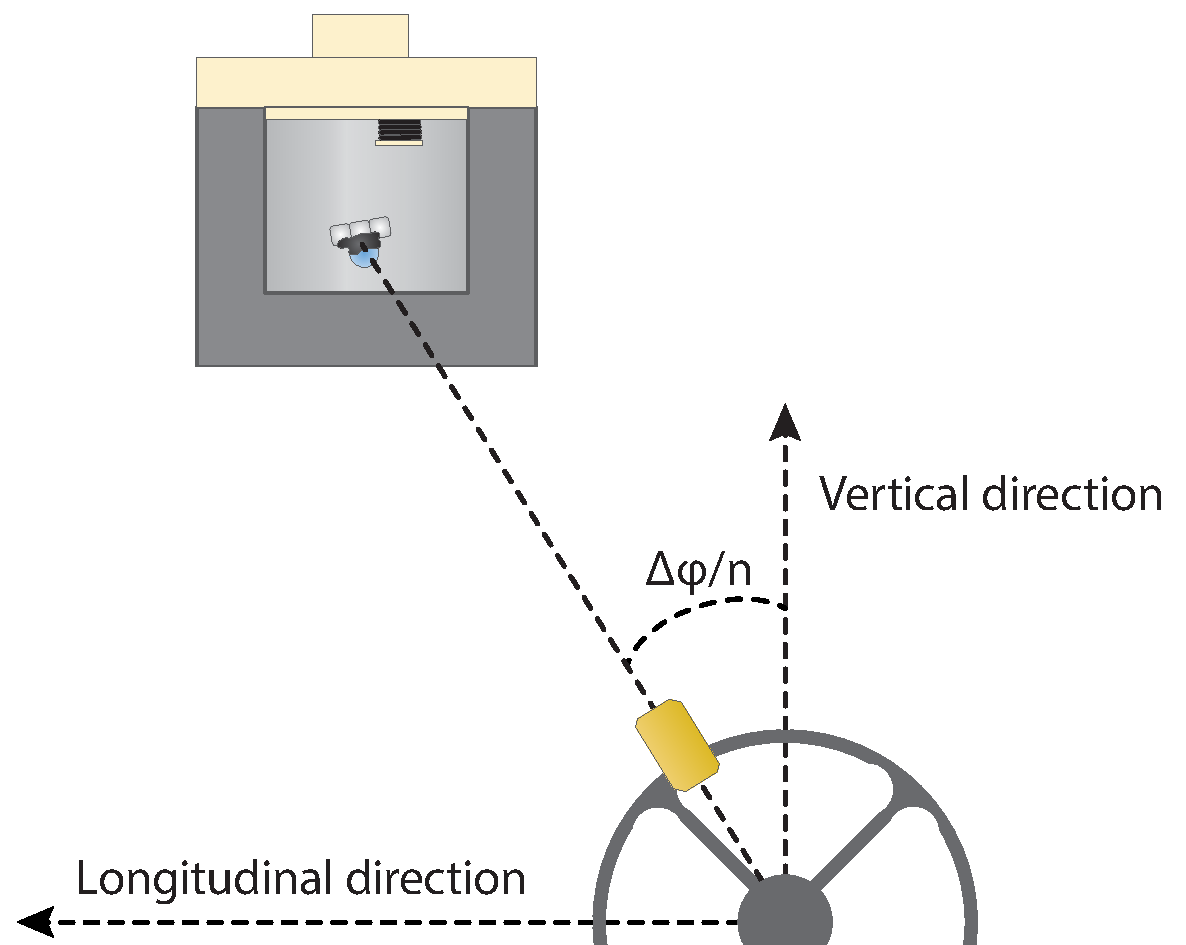
\includegraphics[width=1\textwidth]{Appenidx/paper_wheel_phase.pdf}%, bb=0 0 6000 2000
\caption{\textbf{Schematic depicting the phase angle of the wheel}, as used to define the phase of maximal response in figure 3. Here, $n$ refers to the amount of masses on the wheel, in this case three. This factor follows from the detection not distinguishing between the different masses.}\label{app:phase}
\end{figure}

In figure~\ref{fig_supp:photos} are some photographs of critical elements of the experiment. Namely, (part of) the vibration isolation, the coil used to detect the motion of the particle, the transformer used to calibrate the coupling, the tantalum trap, and the wheel used to source the gravitational signal.

\begin{figure}[ht]
\centering
\includegraphics[width=1\textwidth]{Appenidx/supplement_photos.pdf}%, bb=0 0 6200 5200
\caption{\textbf{Photos of the the experimental apparatus of Fig.1}.\\ \textbf{\emph{A}}: The mass-spring system and the silver wire used for thermalisation of the masses and the experiment, with at the bottom the holder on a small triangular platform to attach the springs. \textbf{\emph{B}}: The coil after the first two layers of five loops were wound around it, with the rest of the cap above. The final pick-up loop consisted of four layers. \textbf{\emph{C}}: A close-up of the calibration transformer, before aluminium shielding was added around it. \textbf{\emph{D}}: The tantalum trap, with the elliptical shape and milling marks visible. \textbf{\emph{E}}: The `mass-wheel' as used in the experiments to show gravitational coupling. The three brass masses are placed in an equilateral triangle. Not shown is the laser-photodiode combination used to read out the frequency of the masses. The wheel is surrounded with one centimeter thick steel plates and is attached to a bridge made out of MK-profiles, which is used to control the elevation and positioning of the wheel in the lab relative to the trap inside the cryostat.}\label{fig_supp:photos}
\end{figure}

\clearpage

\section{Determination of decay time, damping factor, and the quality factor of the mechanical modes}
\label{app:qfactortransfer}
The exponential decay time (\texttau) of each mode was determined through ringdown measurements at high amplitude. At low vibrational amplitude, the measured \texttau\ increases, as is expected from non-linearities in the trapping potential. High amplitude measurements were taken to provide a lower bound on \texttau\ with a high signal-to-noise ratio. We focus on the \SI{27}{Hz} mode, as this is the mode we used to detect our gravitational signal. As discussed in section 2, this mode corresponds most closely to the theoretically expected z-mode frequency. Furthermore, it showed the highest degree of vibrational isolation, which is also as expected given our implemented vibration isolation functions predominantly in z. From the response in phase and amplitude shown in section 2 this is further verified, matching closely to the expected scaling of the z-mode gravitational coupling (both amplitude and phase) under translation of the gravitational source.

\begin{figure}[ht]%
\centering
\includegraphics[width=\textwidth]{Appenidx/paper_ringdown_amp.png}%, bb=0 0 750 300
\caption{\textbf{A typical ringdown of the \SI{27}{Hz} mode}, as performed after a magnetic drive through the calibration transformer. The decay time (\texttau) is extracted from an exponential fit.}\label{fig_supp:ringdown}
\end{figure}

The high amplitude \texttau\ provides a lower bound to the low amplitude \texttau\ of the system. We observe a significant difference in \texttau\ for high and low amplitude, which is explained by a duffing non-linearity in the equations of motion of the resonator. From ringdown measurements, we obtain a lower bound to the decay time of $\tau = \SI{1.09e5}{s}$. The error on the fit of this value is \SI{14.7}{seconds}. At the moment, our understanding of this decay time of individual modes is that it depends strongly on the amplitudes in other modes due to a coupling of the non-linearities. This understanding is limited currently, and a further understanding would require further measurements. To minimise the effect of this false sense of precision (versus accuracy) in the current publication, we will instead truncate the values at three decimals.
With the quality factor (Q) of the resonator defined as

    \begin{equation}
        Q = \pi f \tau 
    \end{equation}

and a frequency of the mode $f = \SI{26.7}{Hz}$, we obtain a quality factor of $Q = \SI{9.06e6}{}$. From \texttau\ we can also determine the damping coefficient of the resonator, which is defined as 

    \begin{equation}
        \gamma = \frac{2}{\tau}
    \end{equation}


which gives a damping in the \SI{27}{Hz} mode of $\gamma = \SI{1.84e{-5}}{s^{-1}}$, or a linewidth of $\gamma/2\pi = \SI{2.92}{\mu Hz}$.

\begin{table}[t]
    \large
    \centering
\begin{tabular}{|c||c|c|} %{|p{2cm}|| p{2cm}|p{2cm}|p{2cm}|} 
 \hline
frequency [Hz] & tau [s] & Q factor\\ [0.5ex] 
 \hline%\hline
 15.9 & 3.65$\cdot10^{4}$  & $1.82 \cdot 10^{6}$  \\ 
 \hline
 26.7 & 1.09$\cdot10^{5}$ & $9.13 \cdot 10^{6}$  \\
 \hline
 40.6 & 1.43$\cdot10^{4}$ & $1.82 \cdot 10^{6}$  \\
 \hline
 55.1 & 3.37$\cdot10^{4}$ & $5.84 \cdot 10^{6}$ \\
 \hline
 129 & 0.214$\cdot10^{4}$ & $8.70 \cdot 10^{5}$ \\
 \hline
 147 & 0.152$\cdot10^{4}$ & $6.98 \cdot 10^{5}$ \\
 \hline
\end{tabular}
\caption*{\textbf{Table S1: Tabulated values of the resonator mode parameters.} Again, these values are truncated at at three decimals, since the fit significance of these values is much higher than the actual stability of these values with respect to mode amplitude, as touched upon in the texts. The spring stiffness of the \SI{26.7}{Hz} mode was calculated to be \SI{12}{mN/m}.}\label{tab_supp:tauQ}
\end{table}

\clearpage

\section{Analysis and Calibration of the Single-Stage Particle Readout Circuit and Energy Coupling}
\label{app:calibration}
The motion of the particle, and the resulting force noise of the particle modes, can be calibrated from flux to RMS motion by injecting a magnetic drive through the calibration transformer. The amount of magnetic flux injected is then directly quantised by the SQUID. By measuring the flux induced by the particle response and using the inductance in the circuit and the spring stiffnes, we find a calibration of magnetic flux to motion. 

\begin{figure}[ht]%
\centering
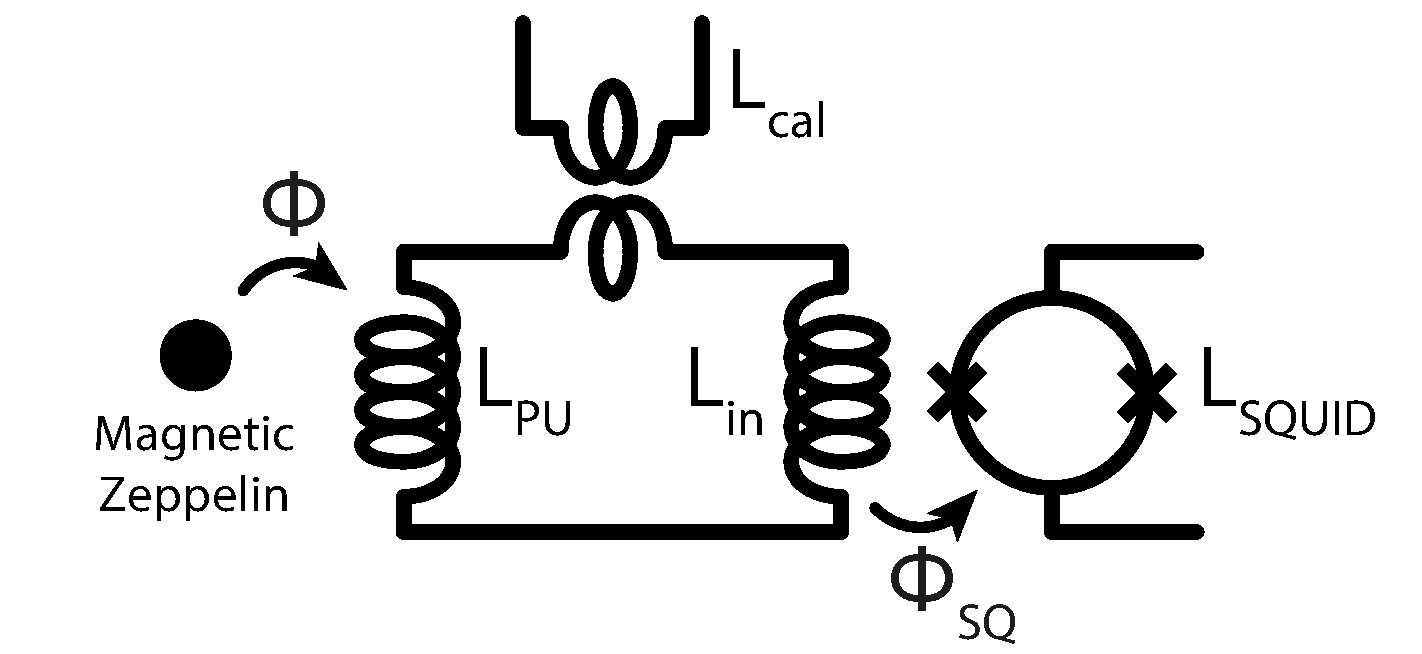
\includegraphics[width=0.5\textwidth]{Appenidx/MLMP_circuit.pdf}%, bb=0 0 680 350
\caption{\textbf{Schematic circuit of the single-stage readout circuit for the magnetic particle }. The transformer used to couple in the external flux used to calibrate the circuit is depicted at the top, with the particle and pick-up loop on the left, and the input coil and SQUID on the right. }\label{fig_supp:readout_circuit}
\end{figure}

This calibration can be intuitively derived from the energy coupling, $\beta^2$. The energy coupling is defined as the fraction of the energies in two coupled oscillating systems, i.e. the amount of energy that couples from one system to the other. This energy coupling is similar to the quality factor of a single system, which is defined as the fraction of energy lost per cycle with respect to the total energy in the system, or equivalently, a measure for the damping of the system. Conversely, the quality factor provides a measure for the maximal energy stored in the resonator as a fraction of the input energy when driven at resonance for a time $T \gg \tau$, that is to say: the energy at which the fractional energy loss per cycle is equal to the energy put in each cycle by the resonant drive. 

For our system, with a mechanical resonator in the form of the trapped magnetic particle, and a driving magnetic field coupled in through the calibration transformer and coupled to the particle through the pick-up loop, we get 

\begin{equation}
    \beta^2 \equiv \frac{L_{total}I^2}{kx^2} 
\end{equation}

with $x$ any spatial coordinate. Going to the limit of infinitesimal displacement, and using $k =m\omega^2$ and using $L_{total}I^2 = \Phi^2/L_{total}$, we obtain

\begin{equation}
    \beta^2 = \frac{\left(\frac{d\Phi}{dx}\right)^2}{L_{total}\cdot m\omega^2}
\end{equation}

from which it is evident that the energy coupling can be used to determine the absolute motion of the magnetic particle from the flux measured in the SQUID.

To measure $\beta^2$, we further consider the motion of the resonator as a simple resonantly driven harmonic oscillator, with the \emph{Ansatz} $x(t) = A(t)e^{i\omega t};\ A(t) = \frac{F}{2 m \omega}\cdot t$, from which we obtain a damping force

\begin{equation}
    F_{damping} \left(= 2 m \zeta \omega_0 \frac{dx}{dt} = \gamma_m v \right)= \gamma_m \cdot\omega\cdot x
\end{equation}

The quality factor Q is equivalently defined as $Q = \frac{1}{2\zeta}$, thus $\gamma_m = \frac{m\omega}{Q}$.
In our calibration procedure, we inject a flux through the calibration transformer. This flux then results in a current through the detection circuit. This current is detected as a flux by the SQUID, with known $\frac{dI}{d\phi}$ calibration from the SQUID parameters. We refer to this current as the the crosstalk current $I_{crosstalk}$. This current also leads to a flux through the pick-up loop, which gives rise to a magnetic force on the particle of the form $F_{drive}=\alpha \cdot I_{crosstalk}$. Here, $\alpha$ is a coupling constant of units $\si{[N/A]}$ that contains a geometrical factor determined by both the relative positioning of the particle with respect to the pick-up coil, and the physical sizes of this coil and particle. As the particle is driven, the motion of the particle will in turn induce a current in the detection circuit. This induced current has the form $I_{induced}=\delta\cdot x$ where $\delta$ is a coupling constant with units $\si{[A/m]}$, which is by symmetry effected through the pick-up coil-particle geometry in the same way that $\alpha$ is.\\
Combining these results, and noting that for the steady state solution the driving force must be equal to the damping force

\begin{equation}
    \frac{I_{induced}}{I_{crosstalk}} =
    \frac{\delta\cdot x}{F_{drive}/\alpha} =
    \frac{\delta \cdot \alpha\cdot x}{\gamma_m \cdot \omega \cdot x} =
    Q\cdot \frac{\alpha\cdot\delta}{m\omega^2} = 
    Q\cdot \frac{\alpha\cdot\delta}{k}
    \label{eq:I/I}
\end{equation}

Since some of our decay times are rather long, in our experiments we work with a $Q_{eff} = \pi fT$, where $T$ is the time during which the drive is applied. Whilst this is not the steady state, this discrepancy is fully absorbed in our definition of $Q_{eff}$:

\begin{equation}
    \frac{I_{induced}}{I_{crosstalk}} =
    \frac{\delta\cdot x}{F_{drive}/\alpha} =
    \frac{\delta \cdot \alpha\cdot x}{\gamma_{eff} \cdot \omega \cdot x} =
    Q_{eff}\cdot \frac{\alpha\cdot\delta}{m\omega^2} = 
    Q_{eff}\cdot \frac{\alpha\cdot\delta}{k}
\end{equation}

From this derivation, we have found that the fraction of the currents in our detection circuit contains all the coupling constants in our system. In fact, looking at the units, we find

\begin{equation}
    \frac{\alpha\cdot\delta}{k} = 
    \frac{\si{\left[\frac{N}{A}\right]}\cdot\si{\left[\frac{A}{m}\right]}}{\si{\left[\frac{N}{m}\right]}}
\end{equation}

Furthermore, for small displacements in $x$, the flux change through the pick-up loop can be treated as linear. The resultant current in the detection circuit must then be $I_{induced} = \frac{d\Phi}{dx}\cdot x \cdot \frac{1}{L_{total}}$ or $\delta = \frac{d\Phi}{dx}\cdot \frac{1}{L_{total}} \hat{=} \si{\left[\frac{A}{m}\right]}$.

As noted before, $\delta$ contains the same geometric scaling as $\alpha$. From the symmetry, we recognise that $\alpha = \frac{d\Phi}{dx}$ ($\left[\SI{}{Wb/m}\right]= \left[\SI{}{N/A}\right]$). Combining these results, we find

\begin{equation}
    \frac{\alpha\cdot\delta}{k} = \frac{\left(\frac{d\Phi}{dx}\right)^2}{L_{total}\cdot m\omega^2} = \beta^2
\end{equation}

This final results gives us a measurable result for $\beta^2$, or, conversely, the proportionality constant $\frac{d\Phi}{dx}$ that equates our measured flux to an absolute motion. The calibration measure is then found from 

\begin{equation} \label{eq:dphi_dx_beta}
    \frac{d\Phi}{dx} = \sqrt{L_{total}\cdot m\omega^2\cdot \beta^2} = \sqrt{L_{total}\cdot m\omega^2\cdot \frac{I_{induced}}{Q\cdot I_{crosstalk}}} 
\end{equation} 

Noting that both $I_{induced}$ and $I_{crosstalk}$ are converted equally by the SQUID, the measured voltage can be inserted for the current through the detection circuit, which provides our sensitivity as 

\begin{equation}
    \frac{d\Phi}{dx} = \sqrt{L_{total}\cdot m\omega^2\cdot \frac{\Delta V_{drive}}{Q\cdot V_{crosstalk}}}
\end{equation}

Here $\Phi$ is the flux through the pick-up loop. Since we detect this using the SQUID, we need to convert this value to the flux through the SQUID, which is done by dividing by the total inductance of the circuit and multiplying by the mutual inductance of the SQUID input loop and the SQUID loop. As a final step, this value can be related directly to the voltage measures made by taking the SQUID gain value as measured.  

\begin{equation}
    \frac{dV}{dx} = 
    \frac{dV}{d\Phi_{SQ}}\cdot\frac{d\Phi_{SQ}}{dI}\cdot\frac{dI}{d\Phi}\cdot\frac{d\Phi}{dx} =
    \frac{dV}{d\Phi_{SQ}} \cdot M_{in,SQ} \cdot \frac{1}{L_{total}}\cdot \frac{d\Phi}{dx}
\end{equation}

The values for the inductances in $L_{total} = L_{PU}+L_{TP}+L_{input}+L_{calibration}$ are: $L_{PU} = \SI{2.9e{-7}}{H}$ the inductance of the pick-up loop, $L_{TP} = \SI{1e{-7}}{H}$ the inductance of the \SI{10}{cm} superconducting twisted-pair connecting the SQUID input to the pick-up loop, $L_{input} = \SI{4e{-7}}{H}$ the inductance of the input coil of the two-stage SQUID device, and $L_{calibration} = \SI{2e{-9}}{H}$ the inductance of the small calibration transformer coil. For the mutual inductance, the SQUID is calibrated to a value of $M_{in,SQ}^{-1} = \SI{0.5}{\mu A/\Phi_0}$. The SQUID voltage gain is measured as $dV/d\Phi_0 = \SI{0.43}{V/\Phi_0}$. These values, combined with measures of these ring-up's, gives us a value of $\frac{dV}{dx} = \SI{0.16}{{\frac{V}{\mu m}}}$ for the $\SI{27}{Hz}$ mode, with a relative error of 7\%, which is dominated by the error in the voltage calibration measurement. 

\newpage

\section{Comparison to basic Optomechanical Quantities}
Given the vast previous work in the field of optomechanics, we aim to provide a rough outline of how the work presented in this paper compares to quantities in optomechanical experiments, in this appendix. For a more complete treatise of optomechanics and specifically a comparison to magneto-mechanics, we refer to \cite{Romero2021}.

We note that the resonance frequency of our levitated particle corresponds to the frequency of the mechanical oscillator in an optomechanics experiment. At present, our experiment lacks the equivalent of the optical cavity and the light sent to the cavity. It could be added to the experiment, by changing the readout of our experiment. Currently, we use a SQUID based read-out, that relies on DC signals. We could read out the SQUID at higher frequencies (using a GHz cavity). In that case the inductance of the SQUID, which depends on the flux in the SQUID, would provide frequency tuning to a LC resonator, with typical resonance frequencies of 2-20 GHz. 

We adopted $\omega$ to be the frequency of the mechanical resonator, this in contrast to optomechanics, in which $\Omega$ is nominally adopted for the mechanical frequency, with $\omega$ reserved for the optical frequency. In the rest of this appendix, we will refer to the optical frequency as used in optomechanics as $\omega_{opt}$ to avoid confusion.
In the context of optomechanics, the optomechanical coupling, g, is given by the infinitesimal change in wavelength as a function of the change in position of the mechanical oscillator:

    \begin{equation}
        g_{opt} = \frac{d\omega_{opt}}{dx}
    \end{equation}

This is an important quantity that provides a measure on how well the mechanical and optical systems are coupled. Often the value is quoted in terms of the zero-point-motion ($x_{zpm}$) of the resonator, as $g_0$.
In the case of magnetic levitation, a translation from  $\frac{d\Phi}{dx}$ to $\frac{d\omega_{opt}}{dx}$ can be made through the realization that the inductance of the SQUID $L_J=\frac{\Phi_0}{2 \pi I_c(\Phi)}$ depends on the flux through the SQUID. This change in inductance changes the resonance frequency of the LC resonator, $\omega_{LC}$, that could be used to readout our SQUID in the future. In the same way that the resonance frequency of an optical cavity depends on the position of a membrane, we also see that the resonance frequency of the LC circuit that the SQUID is part of, depends on the position of our levitated magnetic particle. 

Combining this with equation~\ref{eq:dphi_dx_beta}, we find:

\begin{equation}
    g_{mag} = \frac{d\omega_{LC}}{d\Phi} \frac{d\Phi}{dx} = \frac{d\omega_{LC}}{d\Phi} \sqrt{L_{total}\cdot m\omega^2\cdot \beta^2}
\end{equation}

Evidently, this is the equivalent to $g_{opt}$ for our SQUID detected system. Implicit in the term $L_{total}$ is the coupling loss from parasitic inductances. 
Since the detection is not resonant, like it would be in an optical cavity system, this remains a negligible loss. 
Expressing $g$ in terms of the resonator zero-point-motion can be done similar to how it is often derived in optomechanical systems, from equating the energy of the bosonic system at zero occupation to the kinetic energy at zero point motion:

\begin{equation}
    x_{zpm} = \sqrt{\frac{\hbar}{2 \cdot m_{eff} \cdot \omega_m}}
\end{equation}

Where $m_{eff}$ is the effective mass of the mechanical oscillator and $\omega_m$ is the frequency of the mechanical oscillator. In our case the $m_{eff}$ is just the mass of the levitated particle and $\omega_m$ is the eigenfrequency of the measurement. Filling in the mass and frequency used in the gravity measurements, a zero point motion of $x_{zpm} = \SI{0.86}{fm}$ can be calculated. Combining this with our measured sensitivity, we find $\frac{d\Phi}{dx} \cdot x_{zpm}= \SI{63}{n\Phi_0}$ as a zero point flux for our system. For a slope, $\frac{d\omega_{LC}}{d\Phi}$,  of a $\lambda/4$ resonator terminated with a SQUID of $\SI{1}{GHz/\Phi_0}$, this results in a $g_{0,mag} = g_{mag} \cdot x_{zpm} = \SI{63}{Hz}$. 
%zero point fluxtuation
We conclude, however, that it will be a considerable challenge to make the Q factor of such a LC resonator high enough to reach the sideband resolved limit.

%\red{Gesprek met Bas: verhouding tussen position noise en zero point motion uitrekenen, dit zegt eigenlijk of je kan meten of iets in ground state is.}


%calc of g_{mag,0}, g_{mag,0}= dPhi/dx, maar die hebben we ook niet in de exel. g_{mag,0}= sqrt(L_tot m w^2 beta^2) * x_{zpf} = sqrt( 7.91e-7 H *0.43mg * (2*pi*26.7Hz)^2 * 2.4628e-6) * sqrt(hbar/(2 * 0.43mg * (2*pi*26.7Hz)))
%https://www.wolframalpha.com/input?i=sqrt%28+7.91e-7+H+*0.43mg+*+%282*pi*26.7Hz%29%5E2+*+2.4628e-6%29+*+sqrt%28hbar%2F%282+*+0.43mg+*+%282*pi*26.7Hz%29%29%29+in+phi_0




\newpage

\section{Correction and Conversion of the Data to Units of \texorpdfstring{$\SI{}{N/\sqrt{Hz}}$}{N/rtHz}}
\label{app:correction_and_conversion}
The data used in our gravitational experiments comes from the photodiode detector which measures the passages of the masses on the wheel, and the SQUID signal. Both these signals are filtered by our lock-in amplifiers. Since our gravity experiments were performed at differing amplitudes in the mode, each time trace had a different slope, as discussed in Supp.~\ref{app:qfactortransfer}. To account for this, we have subtracted an individual exponential decay in the form of $Ae^{t/\tau_{fit}}$ from each.

\begin{figure}[ht]
\centering
\includegraphics[width=\textwidth]{Appenidx/paper_Ringdown_Subtract.png}%, bb=0 0 450 300
\caption{\textbf{Ringdown subtraction as performed on the time trace measurement of each wheel position}. Shown here for a separation between particle and driving mass at wheel phase zero of \SI{48.1}{cm} vertical, and laterally displaced by \SI{3.5}{cm}. Residual plotted in the lower half, where we see the fluctuations as result of the drive up and drive down effected by the mass-wheel, which is slightly detuned in frequency with respect to the mode. We drive detuned since we wish to stay away from the non-linear driving and frequency shift of the mode that happens at large amplitude. Furthermore, detuned driving enables us to substract the absolute amplitude.}%\label{fig_supp:}
\end{figure}

After subtracting the ringdown, we apply a phase factor to the time traces. This phase factor is determined based on the detuning of the resonator frequency with respect to the lock-in center frequency. This change ensures that the central peak of the resonator mode will fall fully in a single bin of the Fourier transform we perform next, this ensures that the transfer function of the resonator mode is fully symmetrical. Before performing the Fourier transform, we also cut out a section of the time trace in which there is an integer amount of phase cycles for the mass-passage signal, which ensures smooth periodic boundary conditions for our FFT.
This results in a spectrum giving us the motion of the particle per root hertz, which can be converted to RMS motion in a specific frequency band by integrating over that frequency bandwidth.

\begin{figure}[ht]
\centering
\includegraphics[width=\textwidth]{Appenidx/paper_transferfunction_and_motion.pdf}%, bb=0 0 800 250
\caption{\textbf{Spectrum of the time trace converted to motional noise, with the transfer function plotted overlaid}. The orange vertical line indicates the resonance frequency of the mode.}%\label{fig_supp:}
\end{figure}

By then subtracting the transfer-function of the mechanical mode from the particle signal, and applying our conversion factor to go from $\Phi_0$ to displacement, and using a spring stiffness $k = m\omega^2$ and a mode bandwidth of $df=Q/f$, we arrive at our force noise spectrum in $\SI{}{N/\sqrt{Hz}}$

\begin{figure}[ht]%
\centering
\includegraphics[width=\textwidth]{Appenidx/paper_spectrum_force.pdf}%, bb=0 0 800 250
\caption{\textbf{Force noise spectrum}. Spectrum of the time trace converted to force noise, the final product of this procedure. The orange vertical line indicates the resonance frequency of the mode.}%\label{fig_supp:}
\end{figure}

The noise floor of this measurement corresponds to a mode temperature of \SI{3}{K}, from $T_{mode} = kx_{RMS}^2/k_B$.

\end{appendices}




\end{document}

% Reviewer 1:
% 1 DENNIS Zet vergelijking optomechanics en force noise in appendix, geef waardes uit review paper. Vermeld dat onze beta een soort van g is.
% 2 REBUTTAL Er is al een verwijzing naar Andrea, kunnen misschien wel zeggen dat wij etsen/ surface finishing.
% 3 REBUTTAL Zijn we mee bezig, wordt future paper. Zijn van plan xy vibis te doen.


% Reviewer 2:
% 1 REBUTTAL Wij hebben vrij veel onzekerheid door zwaartekracht op de houder, onzekerheid op plaatsing, onzekerheid afstand tot trap, onzekerheid massa magneet. Wij gaan een fit doen en die waarde gebruiken. Daarbij ook de sigma van G geven, error prop geeft 36% error (=hoog).
% 2 REBUTTAL Dit is een proof of principle, volgende stap is inderdaad naar 2 zulke massa's gaan.
% 3 REBUTTAL Effectieve massa van dit soort oscilatoren is vaak veel kleiner dan daadwerkelijke massa membraan, verder zitten die vaak in hoog frequentiegebied. Tim is benieuwd welke van dit soort oscillatoren een Q factor hebben van hoger dan 1E7. Hebben we ook al een review voor aangehaald.
% 4 TIM Gaat tim zo in 5 minuten doen.
% 5 TIM stuurt Hendrik en Andrea een mailtje met vraag over gravitational decoherence models.
% 6 JAIMY gaat het weer een keertje doorlezen.


%To do: 11-10-23 Na sessie van Tim en Dennis
1. KLAAR: Dennis: Figuur 3 moet opnieuw geplot worden met de factor 0.4 die uit de fit kwam, ipv de 3/8. De caption moet dan ook aangepast worden. In de tekst wordt dit al besproken.
2. KLAAR:Tim: Tim heeft de tekst voor de rebuttals geschreven
3. Tim: Het stukje van Andrea moet er nog in
4. Jaimy: Was Jaimy door alles heen gekomen met proofreaden?
5. Dennis: Data set geisoleerd naar Hendrik voor open access. We kunnen zeggen: alleen de data die nodig is om de plotjes in de paper na te maken. Dus 1 data set van 6 uur om de appendix te doen, en dan gewoon de 8 andere data sets voor de andere punten niet, dan zetten we er bij in een readme dat ze die kunnen opvragen, maar in eerste instantie alleen de punten zelf.
6. Dennis: moet please please please de fotos voor de QuCoM
7. KLAAR: Dennis: g0 uitrekenen voor ons.


todo 23-10-23

1: KLAAR: figuur 3 legenda 
2: KLAAR: deltaPhi/3
